\documentclass[11pt,a4paper]{article}

\usepackage[utf8]{inputenc}
\usepackage[T1]{fontenc}
\usepackage[english]{babel}
\usepackage{amsmath,amssymb}
\usepackage{graphicx}
\usepackage{booktabs}
\usepackage{hyperref}
\usepackage{geometry}

\geometry{margin=2.6cm}

\title{RINGEST Paper 2}
\author{Jos\'e Ignacio Mart\'in Gandul}
\date{\today}

\begin{document}

\maketitle

\begin{abstract}
% TODO: redactar
\end{abstract}

\section{Introduction}
% TODO: redactar

\section{Methods and Reproducibility}
All downstream statistical analyses were performed from frozen input tables using version-controlled scripts. The resulting tables and summaries were archived as verified runs, with checksums recorded for all analysis outputs. External catalog metadata were treated as frozen inputs prior to downstream analyses.

\section{Pre-registration T9.2: Population Tail}
% TODO: redactar

\begin{table}[ht]
\centering
\begin{tabular}{lllrrrrrr}
\toprule
cohort & event & verdict\_kerr & max\_abs\_residual & network\_matched\_filter\_snr & population\_tail\_rank & population\_tail\_rank\_combined & population\_tail\_top\_tertile & population\_tail\_top\_tertile\_combined \\
\midrule
T6.6\_O3\_literature & GW150914 & marginal & 1.68252 & 26 & 0.684211 & 0.741379 & True & True \\
T6.6\_O3\_literature & GW170104 & marginal & 1.01506 & 13.8 & 0.210526 & 0.224138 & False & False \\
T6.6\_O3\_literature & GW170814 & marginal & 1.51538 & 17.7 & 0.421053 & 0.448276 & False & False \\
T6.6\_O3\_literature & GW170823 & consistent & 0.669007 & 12.2 & 0.0526316 & 0.0344828 & False & False \\
T6.6\_O3\_literature & GW190408\_181802 & consistent & 0.834112 & 14.6 & 0.368421 & 0.413793 & False & False \\
T6.6\_O3\_literature & GW190421\_213856 & consistent & 0.211324 & 10.7 & 0.631579 & 0.689655 & False & True \\
T6.6\_O3\_literature & GW190503\_185404 & consistent & 0.644042 & 12.2 & 0.263158 & 0.275862 & False & False \\
T6.6\_O3\_literature & GW190512\_180714 & consistent & 0.412344 & 12.7 & 0.789474 & 0.827586 & True & True \\
T6.6\_O3\_literature & GW190513\_205428 & consistent & 0.513585 & 12.5 & 0.578947 & 0.655172 & False & False \\
T6.6\_O3\_literature & GW190519\_153544 & consistent & 0.788284 & 15.9 & 0.894737 & 0.913793 & True & True \\
T6.6\_O3\_literature & GW190521 & consistent & 0.595715 & 14.3 & 1 & 1 & True & True \\
T6.6\_O3\_literature & GW190521\_074359 & marginal & 1.32367 & 25.9 & 0.315789 & 0.362069 & False & False \\
T6.6\_O3\_literature & GW190602\_175927 & marginal & 1.00784 & 13.2 & 0.473684 & 0.551724 & False & False \\
T6.6\_O3\_literature & GW190706\_222641 & consistent & 0.891621 & 13.4 & 0.947368 & 0.965517 & True & True \\
T6.6\_O3\_literature & GW190708\_232457 & marginal & 1.56919 & 13.4 & 0.842105 & 0.862069 & True & True \\
T6.6\_O3\_literature & GW190727\_060333 & consistent & 0.300899 & 11.7 & 0.736842 & 0.793103 & True & True \\
T6.6\_O3\_literature & GW190828\_063405 & consistent & 0.799222 & 16.5 & 0.526316 & 0.603448 & False & False \\
T6.6\_O3\_literature & GW190910\_112807 & consistent & 0.854754 & 14.5 & 0.105263 & 0.0862069 & False & False \\
T6.6\_O3\_literature & GW190915\_235702 & consistent & 0.428192 & 13.1 & 0.157895 & 0.137931 & False & False \\
T8.2a\_GWTC4\_pSEOBNR & GW150914 & consistent & 0.731074 & 26 & 0.9 & 0.741379 & True & True \\
T8.2a\_GWTC4\_pSEOBNR & GW170104 & consistent & 0.278614 & 13.8 & 0.3 & 0.224138 & False & False \\
T8.2a\_GWTC4\_pSEOBNR & GW190519\_153544 & consistent & 0.461706 & 15.9 & 1 & 0.913793 & True & True \\
T8.2a\_GWTC4\_pSEOBNR & GW190521\_074359 & consistent & 0.609538 & 25.9 & 0.5 & 0.362069 & False & False \\
T8.2a\_GWTC4\_pSEOBNR & GW190630\_185205 & consistent & 0.319073 & 16.4 & 0.6 & 0.482759 & False & False \\
T8.2a\_GWTC4\_pSEOBNR & GW190828\_063405 & consistent & 0.821184 & 16.5 & 0.8 & 0.603448 & True & False \\
T8.2a\_GWTC4\_pSEOBNR & GW190910\_112807 & consistent & 0.929017 & 14.5 & 0.1 & 0.0862069 & False & False \\
T8.2a\_GWTC4\_pSEOBNR & GW200129\_065458 & consistent & 0.615598 & 26.8 & 0.7 & 0.517241 & True & False \\
T8.2a\_GWTC4\_pSEOBNR & GW200224\_222234 & consistent & 0.614527 & 20 & 0.4 & 0.310345 & False & False \\
T8.2a\_GWTC4\_pSEOBNR & GW200311\_115853 & consistent & 0.579756 & 17.8 & 0.2 & 0.172414 & False & False \\
\bottomrule
\end{tabular}

\caption{Population-tail statistics used in the T9.2 preregistered NULL audit. % TODO: redactar caption}
\label{tab:t9-population-tail}
\end{table}

\section{Post-hoc T10: SNR-Residual Diagnostic}
% TODO: redactar

\begin{figure}[ht]
\centering
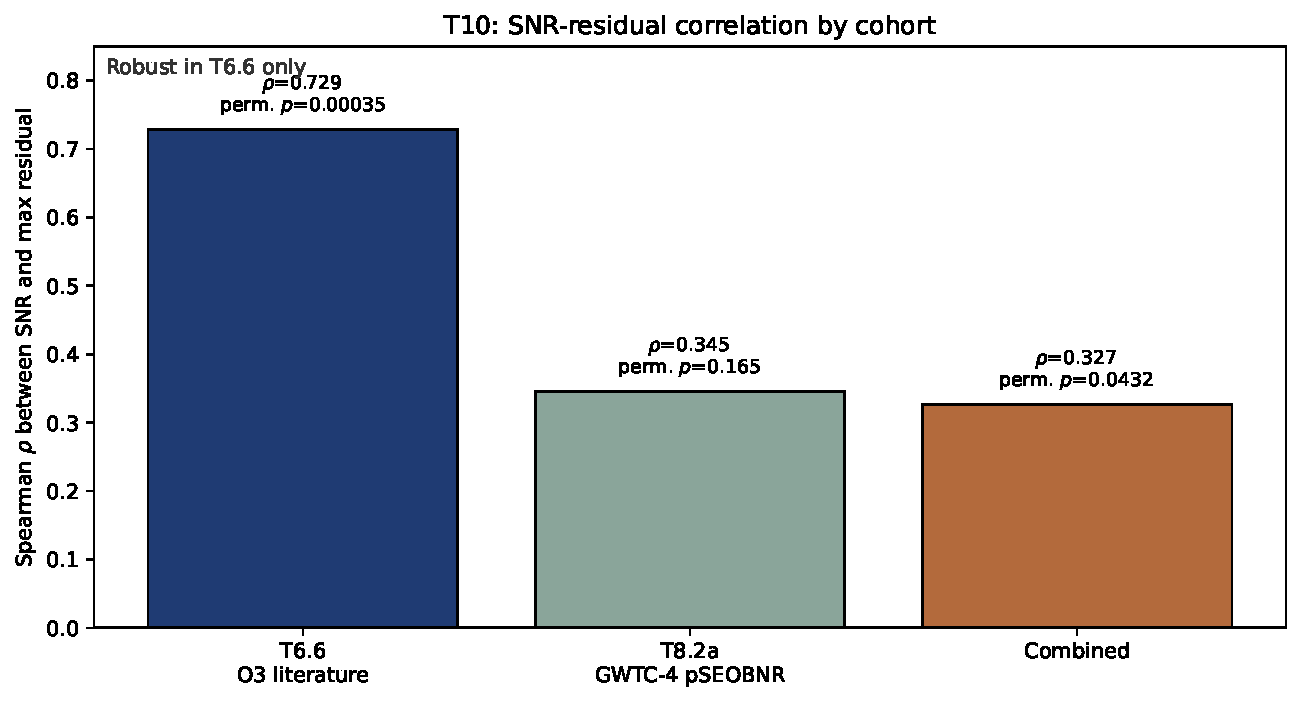
\includegraphics[width=0.82\textwidth]{figures/t10_snr_residual_by_cohort.pdf}
\caption{T10 cohort-level SNR-residual diagnostic. % TODO: redactar caption}
\label{fig:t10-snr-residual}
\end{figure}

\begin{table}[ht]
\centering
\begin{tabular}{lllrrrrrl}
\toprule
cohort & event & verdict\_kerr & max\_abs\_residual & network\_matched\_filter\_snr & snr\_rank\_cohort\_desc & residual\_rank\_cohort\_desc & population\_tail\_rank & audit\_flags \\
\midrule
T6.6\_O3\_literature & GW150914 & marginal & 1.68252 & 26 & 1 & 1 & 0.684211 & TOP3\_SNR\_COHORT;TOP3\_RESIDUAL\_COHORT;TOP5\_SNR\_COMBINED;TOP5\_RESIDUAL\_COMBINED \\
T6.6\_O3\_literature & GW190521\_074359 & marginal & 1.32367 & 25.9 & 2 & 4 & 0.315789 & TOP3\_SNR\_COHORT;TOP5\_SNR\_COMBINED;TOP5\_RESIDUAL\_COMBINED \\
T6.6\_O3\_literature & GW170814 & marginal & 1.51538 & 17.7 & 3 & 3 & 0.421053 & TOP3\_SNR\_COHORT;TOP3\_RESIDUAL\_COHORT;TOP5\_RESIDUAL\_COMBINED \\
T6.6\_O3\_literature & GW190828\_063405 & consistent & 0.799222 & 16.5 & 4 & 10 & 0.526316 &  \\
T6.6\_O3\_literature & GW190519\_153544 & consistent & 0.788284 & 15.9 & 5 & 11 & 0.894737 &  \\
T6.6\_O3\_literature & GW190408\_181802 & consistent & 0.834112 & 14.6 & 6 & 9 & 0.368421 &  \\
T6.6\_O3\_literature & GW190910\_112807 & consistent & 0.854754 & 14.5 & 7 & 8 & 0.105263 &  \\
T6.6\_O3\_literature & GW190521 & consistent & 0.595715 & 14.3 & 8 & 14 & 1 &  \\
T6.6\_O3\_literature & GW170104 & marginal & 1.01506 & 13.8 & 9 & 5 & 0.210526 & TOP5\_RESIDUAL\_COMBINED \\
T6.6\_O3\_literature & GW190706\_222641 & consistent & 0.891621 & 13.4 & 10 & 7 & 0.947368 &  \\
T6.6\_O3\_literature & GW190708\_232457 & marginal & 1.56919 & 13.4 & 11 & 2 & 0.842105 & TOP3\_RESIDUAL\_COHORT;TOP5\_RESIDUAL\_COMBINED \\
T6.6\_O3\_literature & GW190602\_175927 & marginal & 1.00784 & 13.2 & 12 & 6 & 0.473684 &  \\
T6.6\_O3\_literature & GW190915\_235702 & consistent & 0.428192 & 13.1 & 13 & 16 & 0.157895 &  \\
T6.6\_O3\_literature & GW190512\_180714 & consistent & 0.412344 & 12.7 & 14 & 17 & 0.789474 &  \\
T6.6\_O3\_literature & GW190513\_205428 & consistent & 0.513585 & 12.5 & 15 & 15 & 0.578947 &  \\
T6.6\_O3\_literature & GW170823 & consistent & 0.669007 & 12.2 & 16 & 12 & 0.0526316 &  \\
T6.6\_O3\_literature & GW190503\_185404 & consistent & 0.644042 & 12.2 & 17 & 13 & 0.263158 &  \\
T6.6\_O3\_literature & GW190727\_060333 & consistent & 0.300899 & 11.7 & 18 & 18 & 0.736842 &  \\
T6.6\_O3\_literature & GW190421\_213856 & consistent & 0.211324 & 10.7 & 19 & 19 & 0.631579 &  \\
T8.2a\_GWTC4\_pSEOBNR & GW200129\_065458 & consistent & 0.615598 & 26.8 & 1 & 4 & 0.7 & TOP3\_SNR\_COHORT;TOP5\_SNR\_COMBINED \\
T8.2a\_GWTC4\_pSEOBNR & GW150914 & consistent & 0.731074 & 26 & 2 & 3 & 0.9 & TOP3\_SNR\_COHORT;TOP3\_RESIDUAL\_COHORT;TOP5\_SNR\_COMBINED \\
T8.2a\_GWTC4\_pSEOBNR & GW190521\_074359 & consistent & 0.609538 & 25.9 & 3 & 6 & 0.5 & TOP3\_SNR\_COHORT;TOP5\_SNR\_COMBINED \\
T8.2a\_GWTC4\_pSEOBNR & GW200224\_222234 & consistent & 0.614527 & 20 & 4 & 5 & 0.4 &  \\
T8.2a\_GWTC4\_pSEOBNR & GW200311\_115853 & consistent & 0.579756 & 17.8 & 5 & 7 & 0.2 &  \\
T8.2a\_GWTC4\_pSEOBNR & GW190828\_063405 & consistent & 0.821184 & 16.5 & 6 & 2 & 0.8 & TOP3\_RESIDUAL\_COHORT \\
T8.2a\_GWTC4\_pSEOBNR & GW190630\_185205 & consistent & 0.319073 & 16.4 & 7 & 9 & 0.6 &  \\
T8.2a\_GWTC4\_pSEOBNR & GW190519\_153544 & consistent & 0.461706 & 15.9 & 8 & 8 & 1 &  \\
T8.2a\_GWTC4\_pSEOBNR & GW190910\_112807 & consistent & 0.929017 & 14.5 & 9 & 1 & 0.1 & TOP3\_RESIDUAL\_COHORT \\
T8.2a\_GWTC4\_pSEOBNR & GW170104 & consistent & 0.278614 & 13.8 & 10 & 10 & 0.3 &  \\
\bottomrule
\end{tabular}

\caption{SNR-residual audit rows used for T10. % TODO: redactar caption}
\label{tab:t10-snr-audit}
\end{table}

\section{T10.1 Shapley Decomposition on the Six Shared Events}
% TODO: redactar

\begin{figure}[ht]
\centering
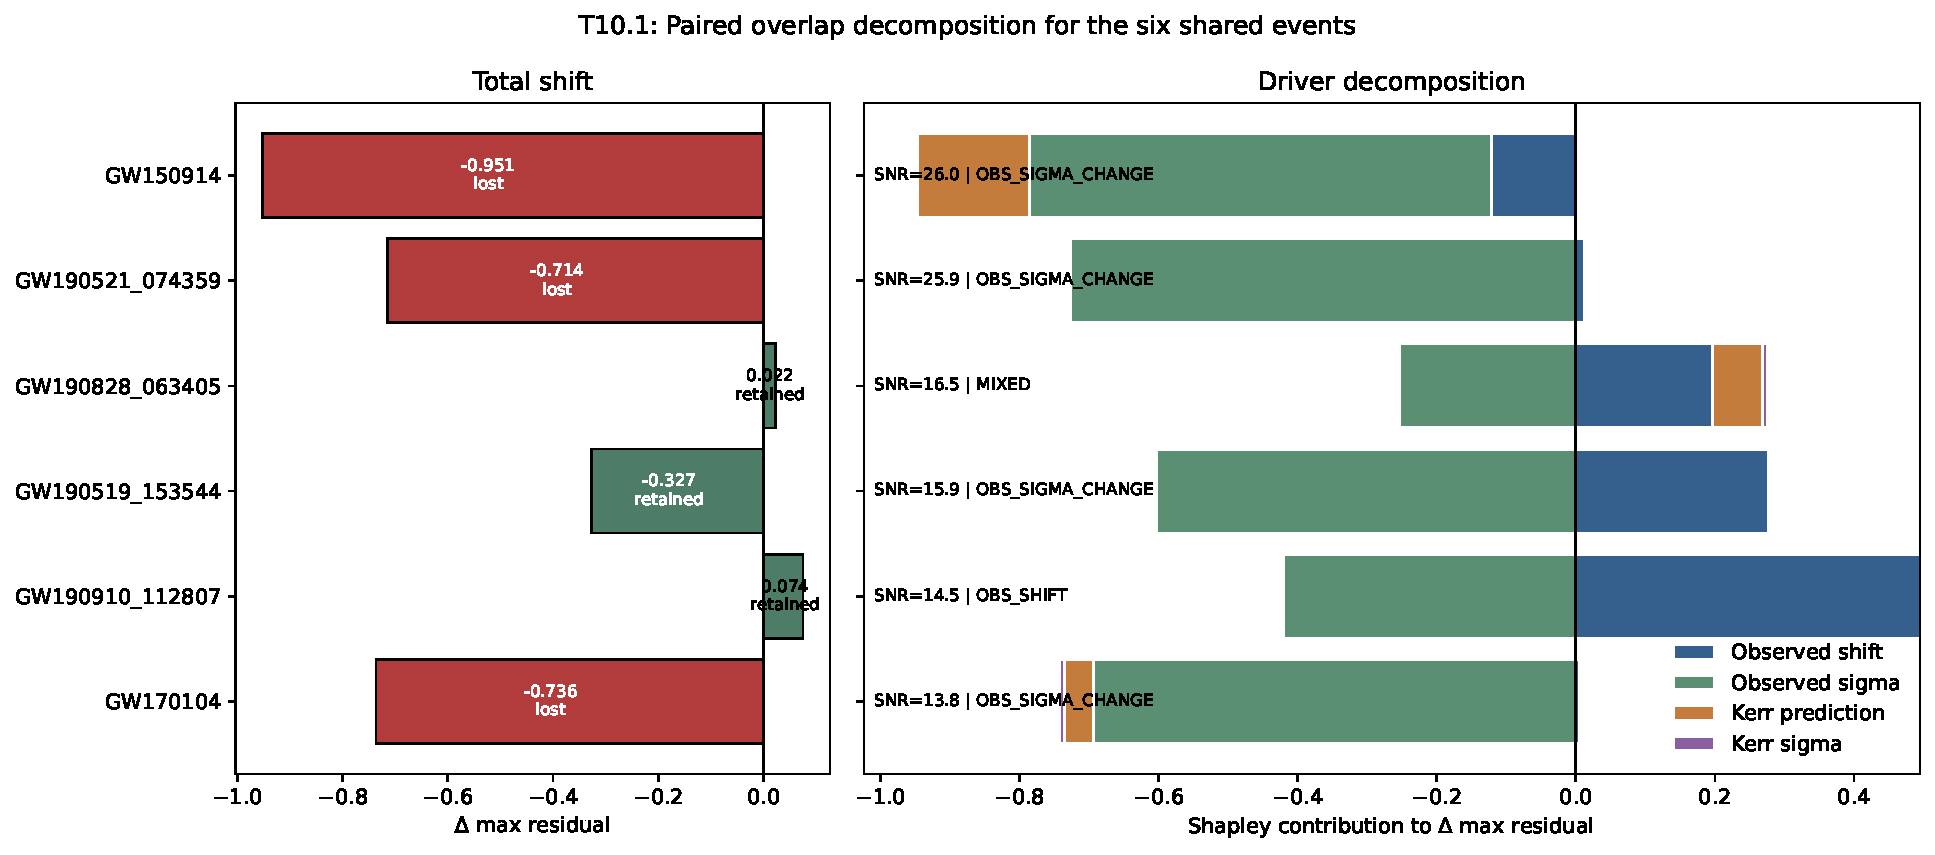
\includegraphics[width=\textwidth]{figures/t10_1_overlap_shapley.pdf}
\caption{T10.1 six-event paired overlap decomposition. % TODO: redactar caption}
\label{fig:t10-1-overlap-shapley}
\end{figure}

\begin{table}[ht]
\centering
\begin{tabular}{lrrrrrrrrlr}
\toprule
event & SNR & max\_abs\_residual\_t66 & max\_abs\_residual\_t82a & delta\_max\_abs\_residual & shapley\_OBS\_SHIFT & shapley\_OBS\_SIGMA\_CHANGE & shapley\_KERR\_PREDICTION\_CHANGE & shapley\_KERR\_SIGMA\_CHANGE & dominant\_driver & lost\_high\_tail\_in\_t82a \\
\midrule
GW150914 & 26 & 1.68252 & 0.731074 & -0.951451 & -0.121349 & -0.664008 & -0.161931 & -0.00416261 & OBS\_SIGMA\_CHANGE & True \\
GW190521\_074359 & 25.9 & 1.32367 & 0.609538 & -0.714134 & 0.0118808 & -0.726014 & 0 & 0 & OBS\_SIGMA\_CHANGE & True \\
GW190828\_063405 & 16.5 & 0.799222 & 0.821184 & 0.0219613 & 0.196104 & -0.25362 & 0.0727909 & 0.00668689 & MIXED & False \\
GW190519\_153544 & 15.9 & 0.788284 & 0.461706 & -0.326577 & 0.276997 & -0.603575 & 0 & 0 & OBS\_SIGMA\_CHANGE & False \\
GW190910\_112807 & 14.5 & 0.854754 & 0.929017 & 0.0742639 & 0.495029 & -0.420765 & 0 & 0 & OBS\_SHIFT & False \\
GW170104 & 13.8 & 1.01506 & 0.278614 & -0.736445 & 0.00594533 & -0.692952 & -0.0416432 & -0.00779483 & OBS\_SIGMA\_CHANGE & True \\
\bottomrule
\end{tabular}

\caption{Six-event overlap decomposition used for T10.1. % TODO: redactar caption}
\label{tab:t10-overlap-decomposition}
\end{table}

\section{Source Audit of the Three Critical Events}
% TODO: redactar

\begin{figure}[ht]
\centering
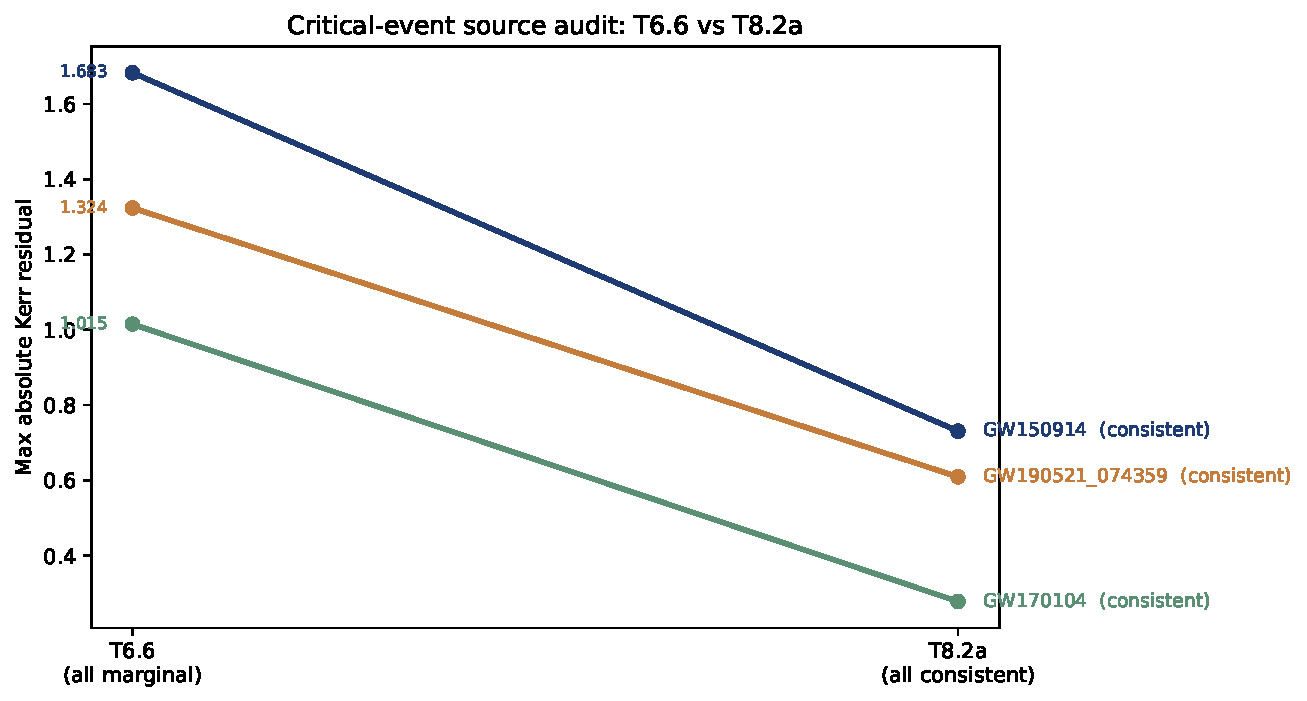
\includegraphics[width=0.82\textwidth]{figures/source_audit_critical_events.pdf}
\caption{Critical-event source audit. % TODO: redactar caption}
\label{fig:source-audit-critical}
\end{figure}

\begin{table}[ht]
\centering
\begin{table}
\caption{Critical-event source audit comparison for T6.6 and T8.2a.}
\label{tab:source-audit-critical}
\begin{tabular}{lrrrlrrrl}
\toprule
event & max\_abs\_residual\_t66 & residual\_f\_t66 & residual\_gamma\_t66 & verdict\_t66 & max\_abs\_residual\_t82a & residual\_f\_t82a & residual\_gamma\_t82a & verdict\_t82a \\
\midrule
GW150914 & 1.68252 & 0.862964 & 1.68252 & marginal & 0.731074 & 0.731074 & 0.18352 & consistent \\
GW170104 & 1.01506 & 0.521482 & 1.01506 & marginal & 0.278614 & 0.227963 & -0.278614 & consistent \\
GW190521\_074359 & 1.32367 & 0.644772 & 1.32367 & marginal & 0.609538 & 0.609538 & 0.402498 & consistent \\
\bottomrule
\end{tabular}
\end{table}

\caption{Critical-event source audit comparison between T6.6 and T8.2a. % TODO: redactar caption}
\label{tab:source-audit-critical}
\end{table}

\section{Final Reading}
% TODO: redactar

\appendix

\section{Supporting Audit Tables}
% TODO: redactar

\begin{table}[ht]
\centering
\begin{tabular}{lrrrrrrrl}
\toprule
event & f\_obs\_hz & f\_kerr\_hz & gamma\_obs\_hz & gamma\_kerr\_hz & residual\_f & residual\_gamma & max\_abs\_residual & verdict\_kerr \\
\midrule
GW150914 & 248 & 233.802 & 238.095 & 203.471 & 0.862964 & 1.68252 & 1.68252 & marginal \\
GW170104 & 287 & 268.97 & 285.714 & 244.901 & 0.521482 & 1.01506 & 1.01506 & marginal \\
GW170814 & 293 & 274.252 & 270.27 & 226.359 & 0.776412 & 1.51538 & 1.51538 & marginal \\
GW170823 & 197 & 186.852 & 181.818 & 154.221 & 0.294448 & 0.669007 & 0.669007 & consistent \\
GW190408\_181802 & 319 & 308.633 & 312.5 & 276.824 & 0.291193 & 0.834112 & 0.834112 & consistent \\
GW190421\_213856 & 162 & 165.099 & 158.73 & 150.326 & -0.0896825 & 0.211324 & 0.211324 & consistent \\
GW190503\_185404 & 191 & 177.385 & 188.679 & 161.512 & 0.399046 & 0.644042 & 0.644042 & consistent \\
GW190512\_180714 & 381 & 390.82 & 384.615 & 361.223 & -0.157487 & 0.412344 & 0.412344 & consistent \\
GW190513\_205428 & 241 & 239.822 & 232.558 & 201.484 & 0.0223248 & 0.513585 & 0.513585 & consistent \\
GW190519\_153544 & 127 & 118.229 & 105.263 & 85.9619 & 0.441596 & 0.788284 & 0.788284 & consistent \\
GW190521 & 68 & 57.1978 & 63.2911 & 55.2871 & 0.595715 & 0.356381 & 0.595715 & consistent \\
GW190521\_074359 & 198 & 185.474 & 185.185 & 155.824 & 0.644772 & 1.32367 & 1.32367 & marginal \\
GW190602\_175927 & 105 & 90.2742 & 100 & 74.5094 & 0.733582 & 1.00784 & 1.00784 & marginal \\
GW190706\_222641 & 108 & 88.9015 & 91.7431 & 65.8402 & 0.745019 & 0.891621 & 0.891621 & consistent \\
GW190708\_232457 & 497 & 443.564 & 476.19 & 391.898 & 1.0099 & 1.56919 & 1.56919 & marginal \\
GW190727\_060333 & 178 & 187.783 & 163.934 & 152.251 & -0.281247 & 0.300899 & 0.300899 & consistent \\
GW190828\_063405 & 239 & 224.617 & 208.333 & 178.882 & 0.429162 & 0.799222 & 0.799222 & consistent \\
GW190910\_112807 & 177 & 167.549 & 169.492 & 145.813 & 0.417545 & 0.854754 & 0.854754 & consistent \\
GW190915\_235702 & 232 & 227.891 & 217.391 & 198.327 & 0.119445 & 0.428192 & 0.428192 & consistent \\
\bottomrule
\end{tabular}

\caption{T6.6 Kerr audit rows used in Phase 2. % TODO: redactar caption}
\label{tab:t66-kerr-audit}
\end{table}

\begin{table}[ht]
\centering
\begin{tabular}{lrrrrrrrl}
\toprule
event & f\_obs\_hz & f\_kerr\_hz & gamma\_obs\_hz & gamma\_kerr\_hz & residual\_f & residual\_gamma & max\_abs\_residual & verdict\_kerr \\
\midrule
GW150914 & 253.3 & 236.238 & 221.729 & 208.721 & 0.731074 & 0.18352 & 0.731074 & consistent \\
GW170104 & 284.8 & 274.069 & 203.666 & 245.822 & 0.227963 & -0.278614 & 0.278614 & consistent \\
GW190519\_153544 & 121.7 & 118.229 & 116.959 & 85.9619 & 0.152523 & 0.461706 & 0.461706 & consistent \\
GW190521\_074359 & 204 & 185.474 & 182.149 & 155.824 & 0.609538 & 0.402498 & 0.609538 & consistent \\
GW190630\_185205 & 247.6 & 242.362 & 262.467 & 207.246 & 0.09667 & 0.319073 & 0.319073 & consistent \\
GW190828\_063405 & 252.4 & 221.687 & 156.006 & 176.549 & 0.821184 & -0.275865 & 0.821184 & consistent \\
GW190910\_112807 & 174.5 & 167.549 & 105.374 & 145.813 & 0.284452 & -0.929017 & 0.929017 & consistent \\
GW200129\_065458 & 247.6 & 232.356 & 196.464 & 188.391 & 0.615598 & 0.117271 & 0.615598 & consistent \\
GW200224\_222234 & 195.8 & 182.013 & 145.138 & 147.573 & 0.614527 & -0.0425364 & 0.614527 & consistent \\
GW200311\_115853 & 239.8 & 221.588 & 190.84 & 192.842 & 0.579756 & -0.00886841 & 0.579756 & consistent \\
\bottomrule
\end{tabular}

\caption{T8.2a Kerr audit rows used in Phase 2. % TODO: redactar caption}
\label{tab:t82a-kerr-audit}
\end{table}

\bibliographystyle{plain}
\bibliography{refs}

\end{document}
